\chapter{Conclusion and perspective of the PhD.}

The original issue addressed in this work is to find an appropriate method to represent emulsion or any ploy disperse multiphase flow within an averaging framework.
Indeed, due to the multiscale physical phenomenon present in those flows it is rather difficult to model the classical governing equations of fluids mechanics.  
Therefore, in this manuscript we presented a clear workflow providing accurate tools for the modeling of multiphase flows. 

We started our presentation by a detailed derivation of the continuous averaged mass, momentum and energy equations, for two arbitrary phases, i.e. no assumption on the topology was made.
Following this, we delved into the statistical approach such as the PBE and kinetics theories.
They were used to model the distribution of particle sizes in disperse multiphase flows
In this context the dispersed phase is modeled as Lagrangian point of mass particles. 
As the latter set of equations was not explicitly linked with the former continuous approach we investigated other ways to model the topology of the dispersed phase. 
Therefore, we first derived a complete Lagrangian framework based on the volume average method. 
Afterward, we demonstrated the equivalence between the continuous and particular averaged equations.
This equivalence principle demonstrated here stipulates that any particular and continuous averaged equations were rigorously equivalent except for the kinematic equations. 
As a result we presented the \textit{no-assumption Hybrid} model, with which it is possible to model the physical and the topology of both phases. 
In conclusion of this first chapter we presented the closure terms of this hybrid model and express the need of numerical simulation to find expression for these closures. 
After a comprehensive review of the numerical studies performed in the literature, we decided to use the open source code \url{http://basilisk.fr} to carry out our own DNS.
In the aim of crafting empirical expression for the closure we set up a mono-disperse rising suspension case in a tri periodic box.
The mesh discretization and statistical convergence were then validated through independence studies. 
A lot of effort have been put on numerical development of these simulations. 
Any user can visit the page \url{http://basilisk.fr/sandbox/fintzin/} to see and use the scripts provided during this PhD. 
Lastly, in \ref{chap:mono-disperse} we present a first glimpse of our results.
We presented all the numerical results together with empirical formula needed to model an oil-water emulsion. 
We limited our study to the closure of the momentum  equation and disregarded the closure related to the changes in topology and poly disperse cases. 

Also, it must be said that extensive researches have been devoted to the study of pairwise collision between the nearest pairs of droplets.
Indeed, we analyzed the DNS results by a Lagrangian tracking of the particles, and we could reconstruct the mean forces and velocity fields around a particle a reference. 
The representation of the velocity and force fields could provide us with some insight on the mean behavior of the particles' interaction. 
By describing with accuracy the behavior of the interactions we are then able to predict if the droplets will coalesce or not depending on the relative initial condition of the droplets and dimensionless parameters. 
Afterward we can derive macroscopic models for the coalescence kernel. 
Although very interesting, it has not been presented in this manuscript yet but only as an oral presentation. 

\section*{Incoming publications}

The work already carried out  is for the most part new and will result in several publications and presentations in conferences. 

The first publication in course of writing is : \textit{The no-assumption hybrid model for poly disperse multiphase flows}
It is focus on the theoretical development of the proof of the equivalence property of the particular and continuous averaged equations, demonstrated in \ref{chap:avg} and \ref{ap:exp}. 
Indeed, after a discussion with prof. Prabu Nott we decided to write a publication on this topic as it might be useful for future theoretical and numerical investigation. 

Regarding the DNS's results we decided to publish one article on the averaged hybrid model momentum  equation's closure presented in \ref{chap:DNS} : \textit{Buoyancy-driven emulsion : part 1 mono-disperse and bi-disperse flows}
Indeed, as a matter of fact there is a gap in the literature regarding the closure terms modeling for emulsions. 
Therefore, accurate close such as the one presented in \ref{chap:DNS} will be of great interest for the community. 
Besides, the study of the impact of the poly dispersion on the closure terms mst be taken into consideration thus we plane to study bi-disperse flows.

The last publication has the temporary title : \textit{A phenomenological description of pairwise interactions in emulsion}. 
This article focus on the statistical description of the closest pair interactions in the  perspective of the development of an accurate coalesce kernel for the hybrid model. 
\begin{figure}
    \centering
    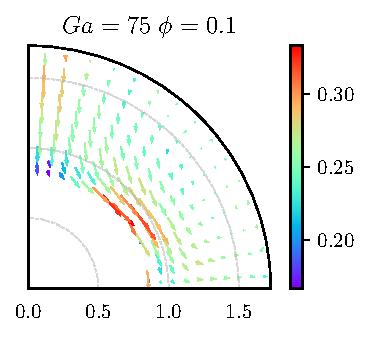
\includegraphics[height=0.35\textwidth]{image/HOMOGENEOUS/fDrop/U_mu_r_0_1_Ga_75_PHI_0_1.pdf}
    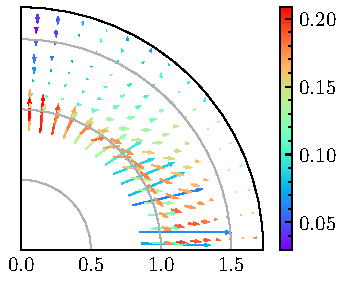
\includegraphics[height=0.35\textwidth]{image/HOMOGENEOUS/fDrop/F_mu_r_0_1_Ga_75_PHI_0_1.pdf}
    \caption{Nearest averaged force fields, $\nstrelavg{\textbf{F}}(\textbf{r})$ for different $Ga$ and $\phi$. 
    Color map : Magnitude of the dimensionless force  $\nstrelavg{\textbf{F}} / (\Delta \rho V g)$.}
    \label{fig:nearestfields}
\end{figure}
\ref{fig:nearestfields} represent the averaged fields of forces and velocities between nearest particles pairs. 
These result permit us to derive a coalescence model based on physical interaction. 


Also, the numerical results related to the statistical analysis of pairwise collisions will be presented at the International Conference on Multiphase Flow (ICMF). 
The Conference will be holds in April 2023 at Kobe (Japan). 

\section*{Future investigations}

Up to now we carried out solely mono disperse DNS. 
Even through these are useful to develop coalesce kernel, they cannot inform us on the effect of the poly dispersion of the flow on the closure quantities. 
So in an additional chapter we will carry out poly disperse simulations of droplets in order to understand how the closure terms behave as a function of the size distribution. 
It turns out that we already have a good idea of which closure term is impacted or not by the topology of the dispersed phase. 
On a second treatment it will be interesting to study the difference between the interaction of different sized droplets. 

On a last point we aim to model three-phase flows, implying that we will perform DNS of emulsion including bubbles within the emulsion. 
In addition to provide additional closure terms, these simulations will help us understand how droplets behave, on average, while interacting with bubbles. 
The industrial benefit is then obvious as we will be able to compute the rate of encapsulation in a water treatment process. 

\section*{Career plan}

After completing my PhD thesis in fundamental fluid mechanics, my personal objective is to continue pursuing research in this field. 
I have a deep passion for understanding the behavior of fluids and the mathematical models that describe their dynamics. 
In my career plan, I envision working in a research-oriented organization where I can contribute to the advancement of knowledge in fluid mechanics. 
My long-term goal is to become an expert in this field and make significant contributions to the development of new theories and technologies. 
I am also interested in teaching and mentoring students who share my interest in fluid mechanics. 
To achieve my career objectives, I plan to stay up-to-date with the latest research and technology, collaborate with other experts in the field, and seek funding opportunities to support my research